\chapter[Metodología de Trabajo]{Metodología de Trabajo}
\label{cp:methodology}

\parindent0pt

Para llevar a cabo los objetivos propuestos en este trabajo final se define una metodología consistente que permita planificar y gestionar las diferentes tareas y recursos de manera ordenada. Este capítulo detalla la planificación del plan de trabajo y el desglose de actividades a través de las cuales se pretende llegar a obtener resultados (Sección \ref{sec:thesis-plan}). Luego se describe la metodología de investigación elegida para el estudio del estado del arte del reciclado de vidrio y la adopción de tecnología blockchain (Sección \ref{sec:research-method}). Finalmente, se describe la metodología de desarrollo del prototipo tecnológico, comprendiendo las etapas de análisis de requerimientos, diseño, implementación, pruebas y despliegue (Sección \ref{sec:software-method}).

\section{Planificación del Plan de Trabajo}
\label{sec:thesis-plan}

En esta sección se describen todos los pasos establecidos como parte del proceso necesario para desarrollar el prototipo basado en blockchain orientado a la trazabilidad y valorización del vidrio. En la Figura \ref{fig:activities-plan} se pueden observar las actividades que conforman el plan de trabajo para cumplir este objetivo. En primer lugar, comienza la formación (Actividad A) estudiando las bases de blockchain y los lenguajes de desarrollo asociados para poder discernir aquellas herramientas tecnológicas que sean más adecuadas para el desarrollo del software propuesto. Conforme avance el tiempo del trabajo final de grado se investigan los pormenores del reciclado, en particular, en el contexto regional de Mendoza (Actividad B). Una vez analizado el estado del arte y las tecnologías asociadas, se selecciona la metodología de trabajo que mejor se adapte al proceso de desarrollar software enfocado en trazabilidad y teniendo en cuenta las características únicas de utilizar blockchain (Actividad C). El proceso de desarrollo de software para una aplicación de trazabilidad sigue una serie de etapas planificadas y estructuradas para asegurar que el producto final cumple con los requerimientos y expectativas, como cualquier otro software, por ende es necesario cumplimentar la serie de etapas previamente definidas en la Actividad C. Luego de seleccionar la metodología, se dedica un periodo de tiempo exclusivamente a las actividades relacionadas con el desarrollo de la aplicación prototipo (Actividad D): análisis de requisitos, diseño del sistema, implementación de los requerimientos, pruebas y validación y finalmente reimplementación si fuera necesario hasta alcanzar el despliegue final. Todo el proceso anteriormente descrito puede llegar a pasar por diferentes iteraciones de progreso si fuera necesario. Finalmente, este trabajo concluye con la escritura del documento final de tesina donde se registra el proceso ejecutado y los resultados alcanzados (Actividad E).

\begin{itemize}
	\item \textbf{Actividad A}: completar la formación en blockchain y las tecnologías y plataformas relacionadas.
	\item \textbf{Actividad B}: realizar un estudio pormenorizado del estado actual del arte en todo lo relacionado con blockchain en el campo del reciclado. En particular, se orienta la búsqueda al reciclado de vidrio. Se analizan trabajos de la literatura como también aplicaciones blockchain orientadas al tema (en caso de existir).
	\item \textbf{Actividad C}: definir los procesos de desarrollo del prototipo, haciendo hincapié en seguir los fundamentos de la ingeniería de software y planificando de forma concisa y clara.
	\item \textbf{Actividad D}: desarrollar la aplicación prototipo. Este desarrollo a su vez involucra las diferentes etapas de un proceso de desarrollo de software, desde análisis de requerimientos, diseño, implementación, evaluación, corrección del prototipo y despliegue. Todos estos pasos se aplican siguiendo una metodología específica, teniendo en cuenta las características particulares del sistema y que además permite llevar a cabo el objetivo general.
	\item \textbf{Actividad E}: Documentar en una memoria el proceso y resultados del trabajo realizado.
\end{itemize}

\begin{figure}[!htpb]
    \centering
    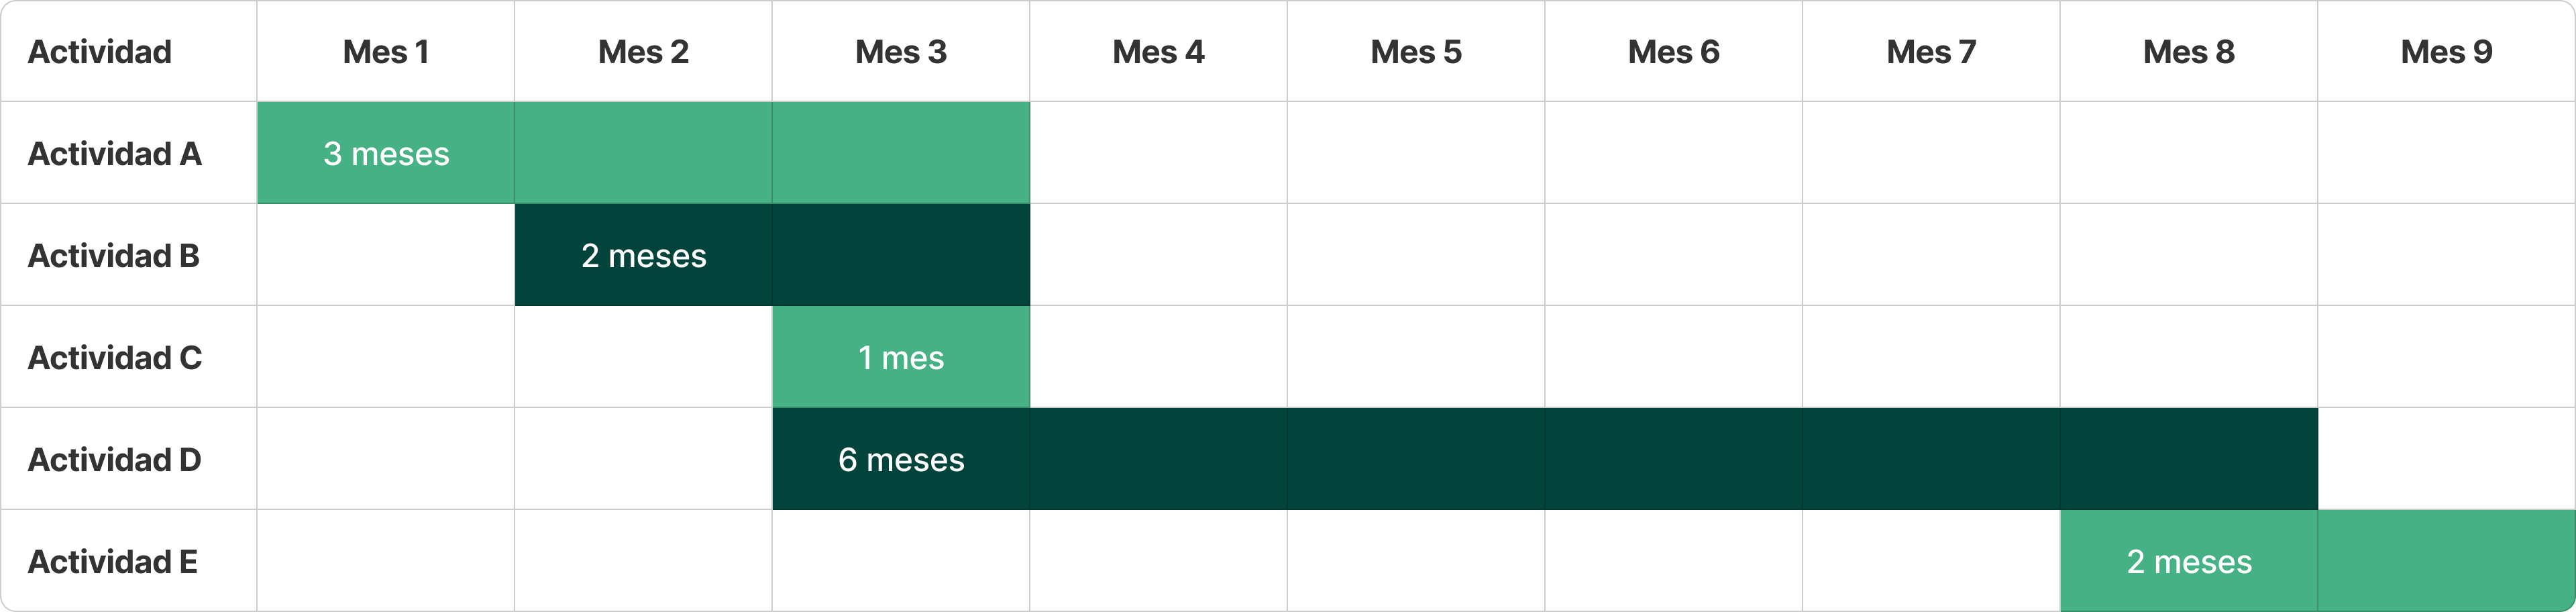
\includegraphics[width=0.8\textwidth]{Figures/activities-plan.png}
    \caption{Planificación de las actividades del plan de trabajo}
    \label{fig:activities-plan}
\end{figure}

En la Sección \ref{sec:research-method} se detalla la metodología de investigación para llevar a cabo la Actividad B de estudio del estado del arte. Luego, en la Sección \ref{sec:software-method} se describe la metodología de trabajo elegida para el proceso de desarrollo del prototipo tecnológico.

\section{Metodología de Investigación}
\label{sec:research-method}

Para llevar a cabo la Actividad B, referida al estudio pormenorizado del estado del arte en blockchain y reciclado de vidrio, se adopta un enfoque de investigación mixto, que combina la revisión sistemática de la literatura con la investigación de campo, incluyendo entrevistas y observaciones. Se selecciona esta metodología con el objetivo de comprender a profundidad el panorama actual de la aplicación de tecnologías emergentes en la gestión de residuos, identificando las tendencias, oportunidades y desafíos específicos del sector del vidrio, tanto a nivel global como en el contexto regional de Mendoza.

La recolección de datos se estructura en dos componentes principales: una revisión exhaustiva de la literatura académica y de proyectos aplicados, y la realización de investigación de campo mediante entrevistas y observaciones.

\subsection{Revisión de la Literatura y Proyectos Aplicados}

Dentro del marco de este trabajo, se realiza una investigación bibliográfica antes del desarrollo técnico, y nuevamente al finalizarlo para la redacción del informe. Se consultan bases de datos como Google Scholar, priorizando artículos de los últimos años, preferentemente desde 2022 en adelante, para asegurar la actualidad de la información. Las palabras clave utilizadas incluyen ``blockchain``, ``supply-chain``, ``waste-management``, ``traceability``, ``smart contracts`` y ``circular economy``, combinadas para afinar los resultados. Se excluyen artículos que no aborden la integración de blockchain con alguna de las otras palabras clave o que sean previos a la fecha límite establecida, salvo casos de particular importancia. La prioridad es identificar estudios que cubran el ciclo completo de la cadena de suministro y el reciclaje. Esta revisión permite identificar los avances tecnológicos, los modelos teóricos propuestos y las brechas existentes en la investigación académica.

Adicionalmente, se lleva a cabo una investigación de proyectos aplicados en el mundo real, buscando soluciones existentes de trazabilidad en cadenas de suministro con blockchain, trazabilidad en reciclaje con blockchain, y sistemas de incentivos para el reciclaje (con o sin blockchain). Estas fuentes secundarias incluyen sitios web de proyectos, informes de organizaciones y artículos periodísticos relevantes. El objetivo es comprender las soluciones prácticas implementadas y sus resultados en diferentes contextos.

\subsection{Investigación de Campo: Contexto Local y Global}

Para obtener una comprensión profunda de la situación del reciclaje de vidrio, particularmente en la provincia de Mendoza, se realiza una investigación de campo. Como punto de partida, se lleva a cabo una revisión en internet de sitios web, artículos de diarios locales y boletines oficiales para documentar programas de reciclaje activos en la región y la presencia de empresas productoras relevantes.

Posteriormente, se realiza una entrevista semiestructurada con Lucía J., responsable del Área de Medio Ambiente de Verallia, la principal empresa productora de envases de vidrio en la región de Mendoza. La entrevista se condujo de manera telefónica, utilizando preguntas guía predefinidas, pero con flexibilidad para explorar temas emergentes durante la conversación. La conversación fue grabada con consentimiento previo y luego transcripta, complementándose con notas tomadas durante la entrevista. Los detalles de esta entrevista se incluyen en el Apéndice \ref{cp:verallia-interview}.

De manera oportuna, y aunque no es el motivo principal de este trabajo, se aprovecha una oportunidad profesional para realizar un viaje de investigación de dos semanas a Europa. Durante este viaje, se visitaron y estudiaron sistemas de reciclaje y programas de incentivos de reciclaje en tres países europeos. Las actividades incluyeron visitas a centros verdes, interacciones con organizaciones involucradas en el reciclaje, exploración de redes de comercios circulares u orientadas a la sustentabilidad, y encuentros con organizaciones dedicadas a promover la economía circular. Los hallazgos y observaciones de este viaje, documentados a través de notas y fotografías, se detallan en el Apéndice \ref{cp:europe-trip}.

\subsection{Procesamiento y Análisis de Datos}
La información recolectada de la literatura se organiza en un inventario de artículos, registrando su título, año, autor, palabras clave y principales aportes. Junto con los hallazgos de la investigación de proyectos aplicados, esta información fue sintetizada, resumida y redactada en el Marco Teórico (Sección \ref{cp:theoretical-framework}), principalmente en la subsección de Proyectos y Trabajos Relacionados (Sección \ref{sec:related-work}).

Para la información cualitativa obtenida de las entrevistas y observaciones en campo, se realiza un análisis de contenido temático. Las transcripciones y notas se revisan para identificar patrones, desafíos y oportunidades relevantes para el reciclaje de vidrio y la aplicación de blockchain en la región. Este análisis permite contrastar la teoría con la realidad local, identificar las necesidades específicas de los actores de la cadena y consolidar la base de conocimiento para la definición de los requisitos y el diseño del prototipo tecnológico.

\subsection{Delimitación del Alcance}

El presente trabajo se centra en la tecnología blockchain como eje principal debido a su naturaleza disruptiva y su potencial para transformar la trazabilidad y la gestión de datos. La elección de la aplicación orientada a la economía circular se justifica por la relevancia actual de este área de impacto y la necesidad de soluciones sostenibles. Particularmente, el dominio se delimita al vidrio, siguiendo la recomendación de investigaciones que sugieren que la especialización en un material particular permite obtener mejores resultados en usabilidad y tasas de reciclaje \cite{pending}. Esto se debe a la posibilidad de diseñar sistemas a medida de los procesos productivos y de reciclaje del material elegido. El vidrio en particular es seleccionado como material reciclable para desarrollar este trabajo por sus características de alta reciclabilidad y su significativo impacto regional en Mendoza (provincia vitivinícola) cuya principal industria productiva, el vino, depende en gran medida de los envases de vidrio. % La localización en Mendoza se debe a que este trabajo se desarrolla en la Universidad Nacional de Cuyo (UNCUYO), con sede principal en esta provincia.

\section{Metodología de Desarrollo}
\label{sec:software-method}

Para llevar a cabo el desarrollo de un prototipo tecnológico que cumpla con los objetivos propuestos en este trabajo resulta necesario definir una metodología consistente que permita planificar y gestionar las diferentes tareas de manera ordenada. Durante la planificación del trabajo, se realizó una comparación de diversas metodologías de desarrollo de software (tradicionales y ágiles) y se hizo una evaluación con el objetivo de seleccionar la metodología más adecuada para las características de este trabajo. El detalle de la comparación y análisis se encuentra en el Apéndice \ref{cp:software-methodology}. 

Como resultado del análisis y comparación de metodologías, se optó por una combinación del modelo en V para la estructura general del proceso de desarrollo de software y Kanban para la gestión de tareas diarias. El modelo en V, que es una extensión del modelo en cascada, está orientado a proyectos con requerimientos bien definidos (poco cambiantes) y donde la validación y verificación son relevantes, como es el caso de un prototipo de trazabilidad basado en blockchain. Este tipo de metodología es apropiada para proyectos basados en blockchain donde la inmutabilidad de los contratos inteligentes requiere una alta calidad y baja tolerancia a errores antes del despliegue. Por otro lado, Kanban se utiliza para gestionar las tareas diarias de manera ágil y flexible, permitiendo adaptarse a cambios menores en el proceso sin comprometer la estructura general del proyecto y sin generar una sobrecarga de trabajo innecesaria. Esta combinación permite mantener un equilibrio entre la estructura sistemática del modelo en V y la flexibilidad operativa de Kanban. Metodologías como Scrum o Extreme Programming (XP) fueron consideradas, pero se descartaron debido a la naturaleza del proyecto y el equipo, ya que en este trabajo no se requiere un enfoque iterativo e incremental tan marcado como el que estas metodologías proponen. Además, metodologías como Scrum requieren roles específicos y reuniones frecuentes que no son necesarias en este contexto, donde el enfoque está más en la planificación y ejecución de un prototipo concreto y definido.

\subsection{Modelo en V}

El desarrollo del prototipo siguió el modelo en V, una metodología de desarrollo de software que extiende el enfoque secuencial del modelo en cascada al emparejar cada fase de desarrollo con una fase de prueba correspondiente, formando una estructura en forma de ``V``. Con esta metodología se asegura una verificación y validación sistemática en cada etapa, permitiendo la detección y corrección temprana de errores y minimizando riesgos al final del proyecto. En la Figura \ref{fig:methodology-v} se ilustran las etapas del proceso. Se observa que los requisitos y componentes del sistema se detallan de forma iterativa en las etapas de la primera mitad descendente de la V. Una vez completada la codificación, el proceso asciende por el lado derecho de la V, donde cada etapa de definición previa es validada a través de pruebas específicas.

\begin{figure}[!htpb]
    \centering
    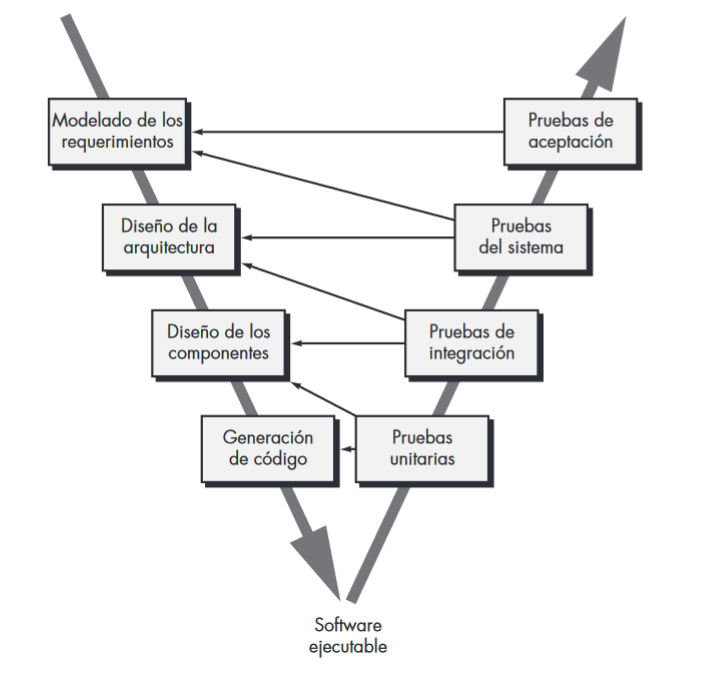
\includegraphics[width=0.6\textwidth]{Figures/model-v.png}
    \caption{Modelo de Desarrollo en V \cite{pressman2010ingeneria}}
    \label{fig:methodology-v}
\end{figure}

% El modelo en V es una opción fuerte para proyectos que requieren altos estándares de calidad y donde los errores tempranos podrían tener consecuencias costosas o críticas. Aunque este modelo comparte algunas limitaciones con el modelo en cascada, como la dificultad para adaptarse a cambios significativos una vez que el proyecto está en curso, su estructura permite una mejor gestión del riesgo y calidad mediante la validación constante de cada etapa del desarrollo.

Las actividades de este trabajo se mapean a las fases del modelo en V de la siguiente manera:

\textbf{Modelado de requerimientos:}
esta fase comprende la identificación y documentación detallada de los requisitos funcionales y no funcionales del prototipo. Los hallazgos se nutren directamente de la Metodología de Investigación previamente definida (Sección \ref{sec:research-method}), que incluye la revisión del estado del arte en blockchain, gestión de residuos y trazabilidad, así como entrevistas y observaciones de programas de reciclaje existentes. El objetivo en esta etapa es comprender las necesidades específicas del sistema de trazabilidad del vidrio para definir un conjunto exhaustivo de requerimientos que aseguren que el prototipo aborde los desafíos identificados en la cadena de producción de envases de vidrio en la región. El resultado de esta fase es un documento de requisitos funcionales y no funcionales que sirve como base para las siguientes etapas del desarrollo. La ejecución y resultados de esta fase se detallan en el Capítulo \ref{cp:modelling}.

\textbf{Diseño (de arquitectura y componentes):}
el diseño del sistema se divide en dos etapas: diseño de arquitectura y diseño de componentes. En la primera etapa, se define la arquitectura general del sistema, incluyendo la selección de tecnologías y plataformas a utilizar, así como la estructura de los módulos principales y la división de responsabilidades entre ellos. En la segunda etapa, se realiza el diseño detallado de cada componente de los módulos del sistema, especificando las interfaces, protocolos de comunicación y estructuras de datos a utilizar. El diseño en etapas y previo a la implementación tiene el objetivo de garantizar que el sistema sea escalable, mantenible y cumpla con los requisitos definidos en la fase anterior. El resultado es un conjunto de documentos de diseño que guían la implementación del prototipo. Los detalles de estas dos fases de diseño se presentan en el Capítulo \ref{cp:design}.

\textbf{Generación de código:}
durante la fase de generación de código o implementación, se lleva a cabo la codificación del prototipo, cada módulo y sus componentes en las tecnologías elegidas y especificaciones detalladas durante la etapa de diseño. Esta etapa es gestionada con el apoyo de Kanban para la organización y seguimiento de las micro-tareas para mantener un flujo de trabajo ágil y adaptable a los cambios menores que puedan surgir durante el desarrollo. El resultado de esta fase es un prototipo funcional que implementa los requisitos y diseños definidos previamente. En simultaneo con la generación de código se realiza la primer etapa de validación, que consiste en pruebas unitarias de cada componente desarrollado. Estas pruebas aseguran que cada componente funcione correctamente de forma aislada y cumpla con los requisitos funcionales especificados. Al finalizar esta etapa, el software ejecutable está listo para ser desplegado en un entorno de pruebas. Los detalles de la implementación y las pruebas unitarias se describen en el Capítulo \ref{cp:implementation}.

\textbf{Pruebas:} 
el proceso de pruebas se lleva a cabo en múltiples etapas. Luego de las pruebas unitarias, se realizan pruebas de integración automatizadas para verificar que los diferentes módulos del sistema interactúan correctamente entre sí a través de sus interfaces. Estas pruebas aseguran que los datos fluyan adecuadamente dentro del sistema. Posteriormente, se llevan a cabo pruebas de sistema para evaluar el comportamiento del prototipo en su conjunto para validar que el sistema cumple con los requisitos funcionales y no funcionales definidos. Las pruebas de sistema incluyen pruebas manuales para validar consistencia de datos en el sistema y que el prototipo cumple con los requerimientos funcionales, mientras que pruebas automatizadas con herramientas permiten verificar los requerimientos no funcionales como rendimiento y seguridad bajo condiciones simuladas. Finalmente, se realizan pruebas de aceptación con un conjunto de usuarios voluntarios para validar que el prototipo cumple con los criterios de aceptación establecidos en la fase de modelado de requerimientos. Los detalles de las pruebas realizadas en estas etapas se presentan en el Capítulo \ref{cp:testing}.

\subsection{Gestión del Proceso}

Para asegurar una gestión eficiente del desarrollo, se implementaron herramientas y prácticas de control de proyectos. La documentación del proceso fue continua a lo largo de todas las fases del ciclo de vida del software. Las decisiones de diseño, problemas encontrados y soluciones aplicadas fueron registradas, sirviendo como base para la elaboración del informe final de tesis. Para el control de versiones del código fuente, se utilizó Git (junto con Github para la gestión de repositorios en la nube), lo que permitió un seguimiento detallado, seguro y ordenado de los cambios. Adicionalmente, se empleó la herramienta Jira para el seguimiento de incidencias, tareas y la evolución general del desarrollo, facilitando la planificación, el monitoreo del progreso, seguimiento de errores detectados y la gestión de tareas pendientes. Esta combinación de herramientas y metodologías permitió mantener un flujo de trabajo organizado, transparente y eficiente, alineado con las necesidades específicas del proyecto.

En los próximos capítulos se detalla el proceso de ejecución llevado a cabo en cada etapa, incluyendo los resultados obtenidos en cada una. En el Capítulo \ref{cp:modelling} se describe el proceso de modelado de requerimientos, donde se explica cómo se obtuvieron los requerimientos funcionales y no funcionales, su priorización y la planificación del desarrollo. En el Capítulo \ref{cp:design} se aborda el diseño del sistema, incluyendo la elección de tecnologías, diseño de arquitectura de software, modelado de la interfaz de usuario y definición de los módulos principales del prototipo. Posteriormente, en el Capítulo \ref{cp:implementation} se detalla la implementación de cada módulo del sistema, integración de los módulos, pruebas unitarias realizadas y despliegue del prototipo en un entorno de pruebas similar a un entorno productivo. En el Capítulo \ref{cp:testing} se describen las pruebas realizadas, tanto las pruebas de integración automatizadas como las pruebas de sistema manuales y las pruebas con usuarios. Finalmente, en el Capítulo \ref{cp:conclusions} se presentan las conclusiones del trabajo, resultados obtenidos, reflexiones sobre el proceso de desarrollo y oportunidades de mejora de este trabajo con recomendaciones para futuros trabajos relacionados con la trazabilidad y valorización del vidrio mediante tecnologías emergentes como blockchain.
